\section{سوال سوم}
برای حل این مسأله ابتدا \lr{maze} به یک گراف تبدیل می‌شود. در گراف هر خانه به خانه‌های اطراف متصل می‌شود به شرطی که مسیر مسدود نباشد. بعد از ساخت گراف برای پیدا کردن مسیر از الگوریتم 
\lr{Depth First Search (DFS)}
استفاده شده‌است. در این الگوریتم به صورت بازگشتی از یک خانه به خانه دیگر می‌رود و ذخیره می‌کند که آیا از این خانه گذشته است یا خیر، که در مراحل دیگر سراغ خانه‌های تکراری نرود. در انتها بعد از رسیدن به مقد مسیر طی شده را بر می‌گرداند. این روش تمامی مسیرهای از مبدأ به مقصد را بر می‌گرداند. با توجه به اینکه هزینه رفتن از هر خانه به خانه دیگر برابر یک (مسیر وزن‌دار نیست) است هزینه را می‌توان به صورت مستقیم خانه‌های طی شده را در نظر گرفت.
کد پیاده‌سازی در الگوریتم \lr{DFS} در فایل \lr{Q3.py} آورده شده است.
 در مجموع ۷۶ مسیر برای رفتن از مبدا به مقصد وجود دارد که تمامی مسیرها در فایل
 \lr{paths.csv}
 آورده شده است. با توجه به اینکه بازه تابع هزینه از ۷ تا ۱۷ است نمی‌توان رتبه ۱۰ و ۵۰ را صرفا یک مسیر مشخص معرفی کرد و حتی برای کمترین هزینه نیز دو مسیر وجود دارد؛ صرفا مسیری که \lr{DFS} بدست آورده و تابع هزینه آن رتبه‌های خواسته شده را داراست، آورده شده است و جواب یکتا ندارد ولی هزینه مسیر یکتا است.
 \begin{figure}[!h]
 	 	\centering
 	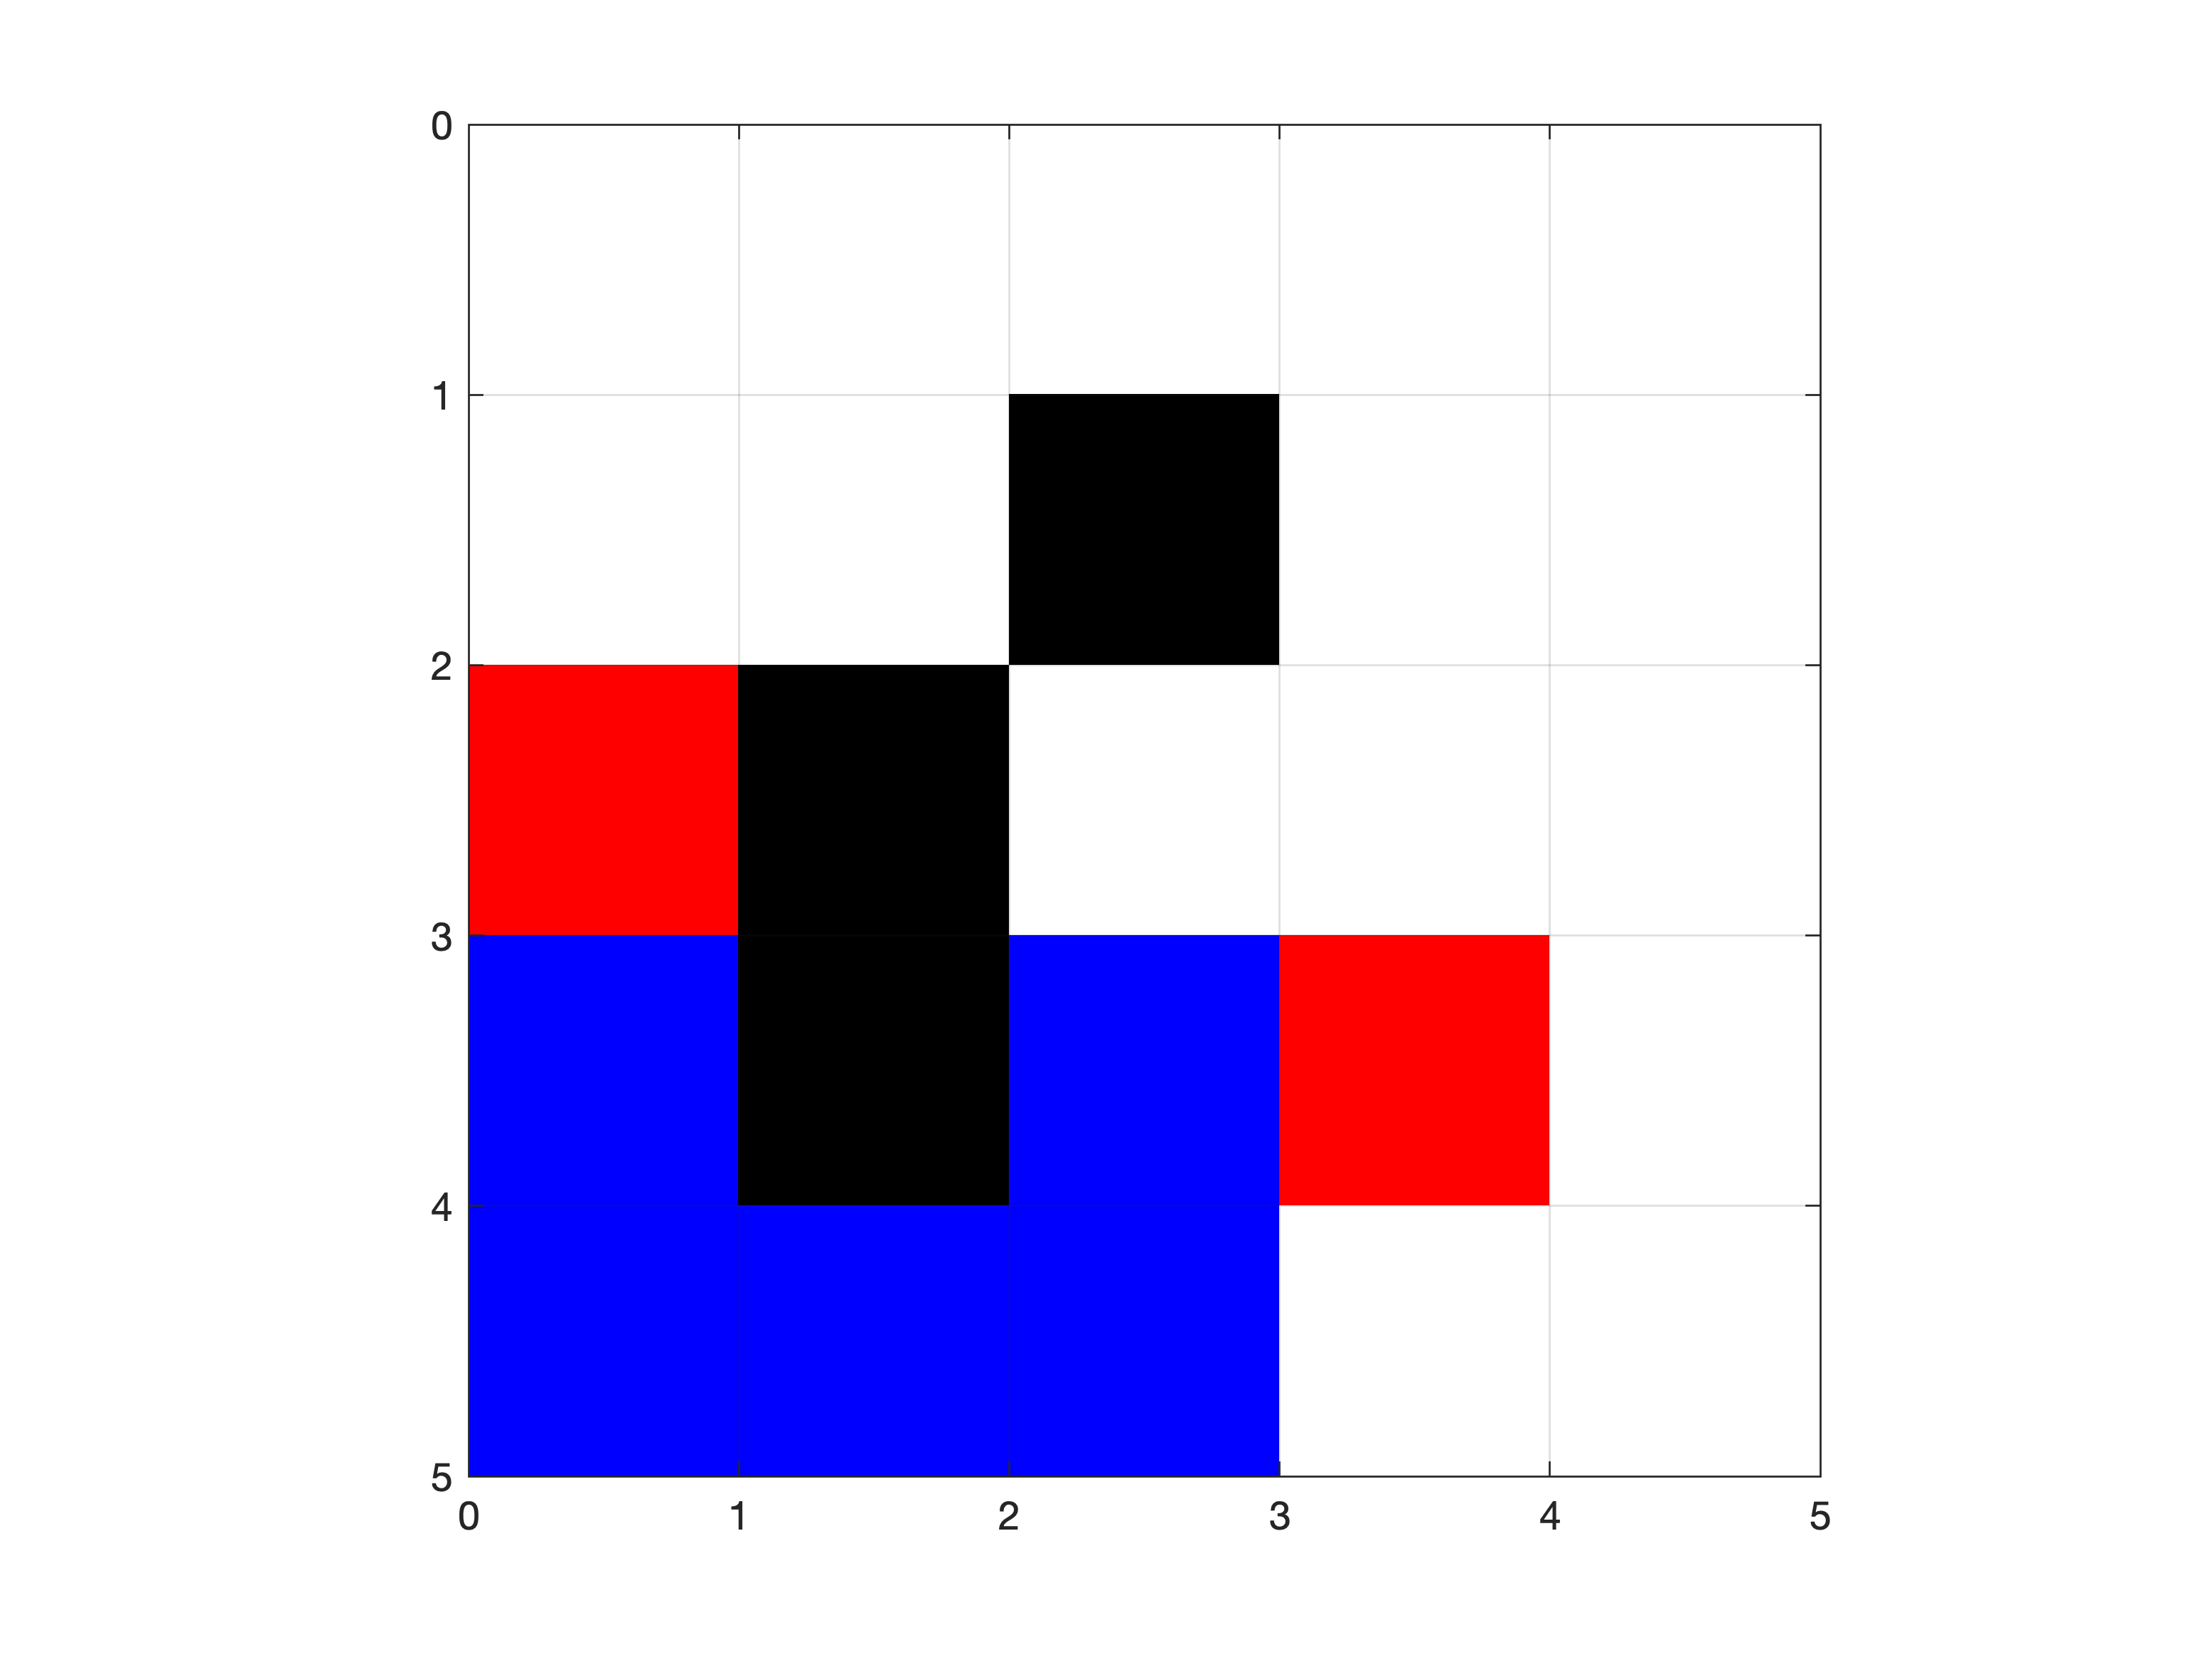
\includegraphics[width=12cm]{../Figure/Q3/1th_path.png}

 	\caption{مسیر با هزینه ۷ و رتبه ۱}
 \end{figure}

 \begin{figure}[!h]
	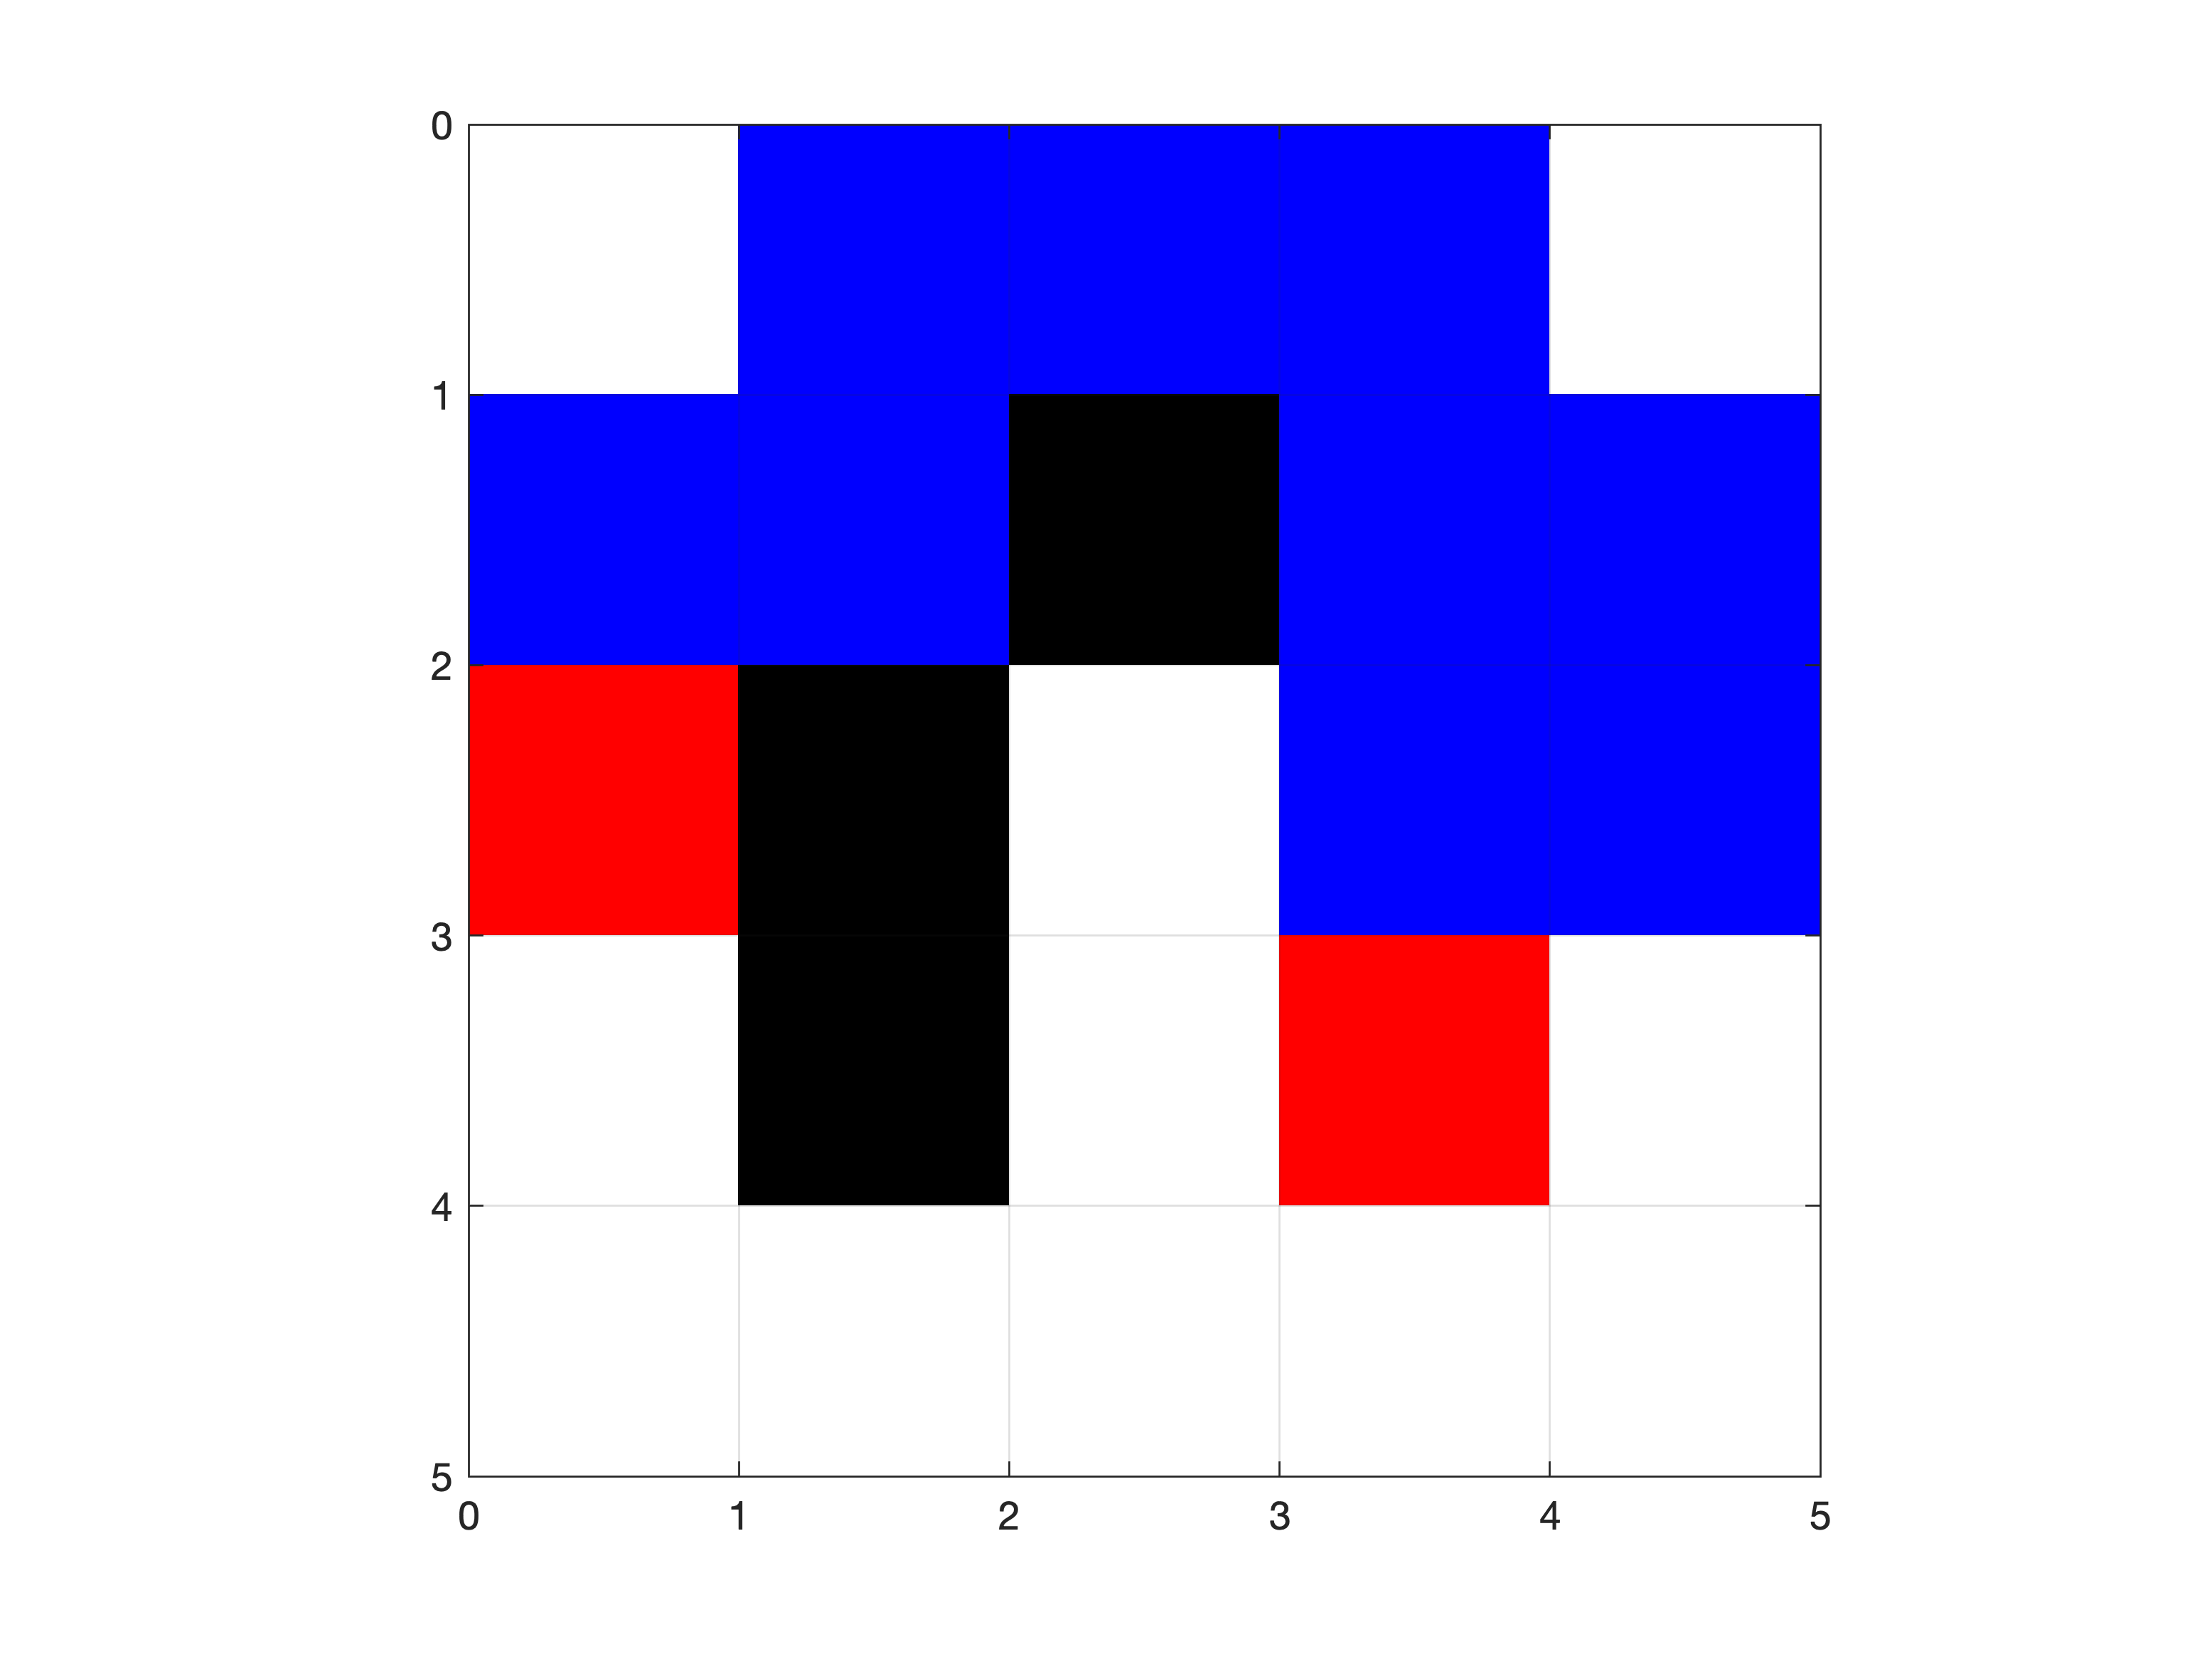
\includegraphics[width=12cm]{../Figure/Q3/10th_path.png}
	\centering
 	\caption{مسیر با هزینه 11 و رتبه ۱۰}
\end{figure}

 \begin{figure}[!h]
	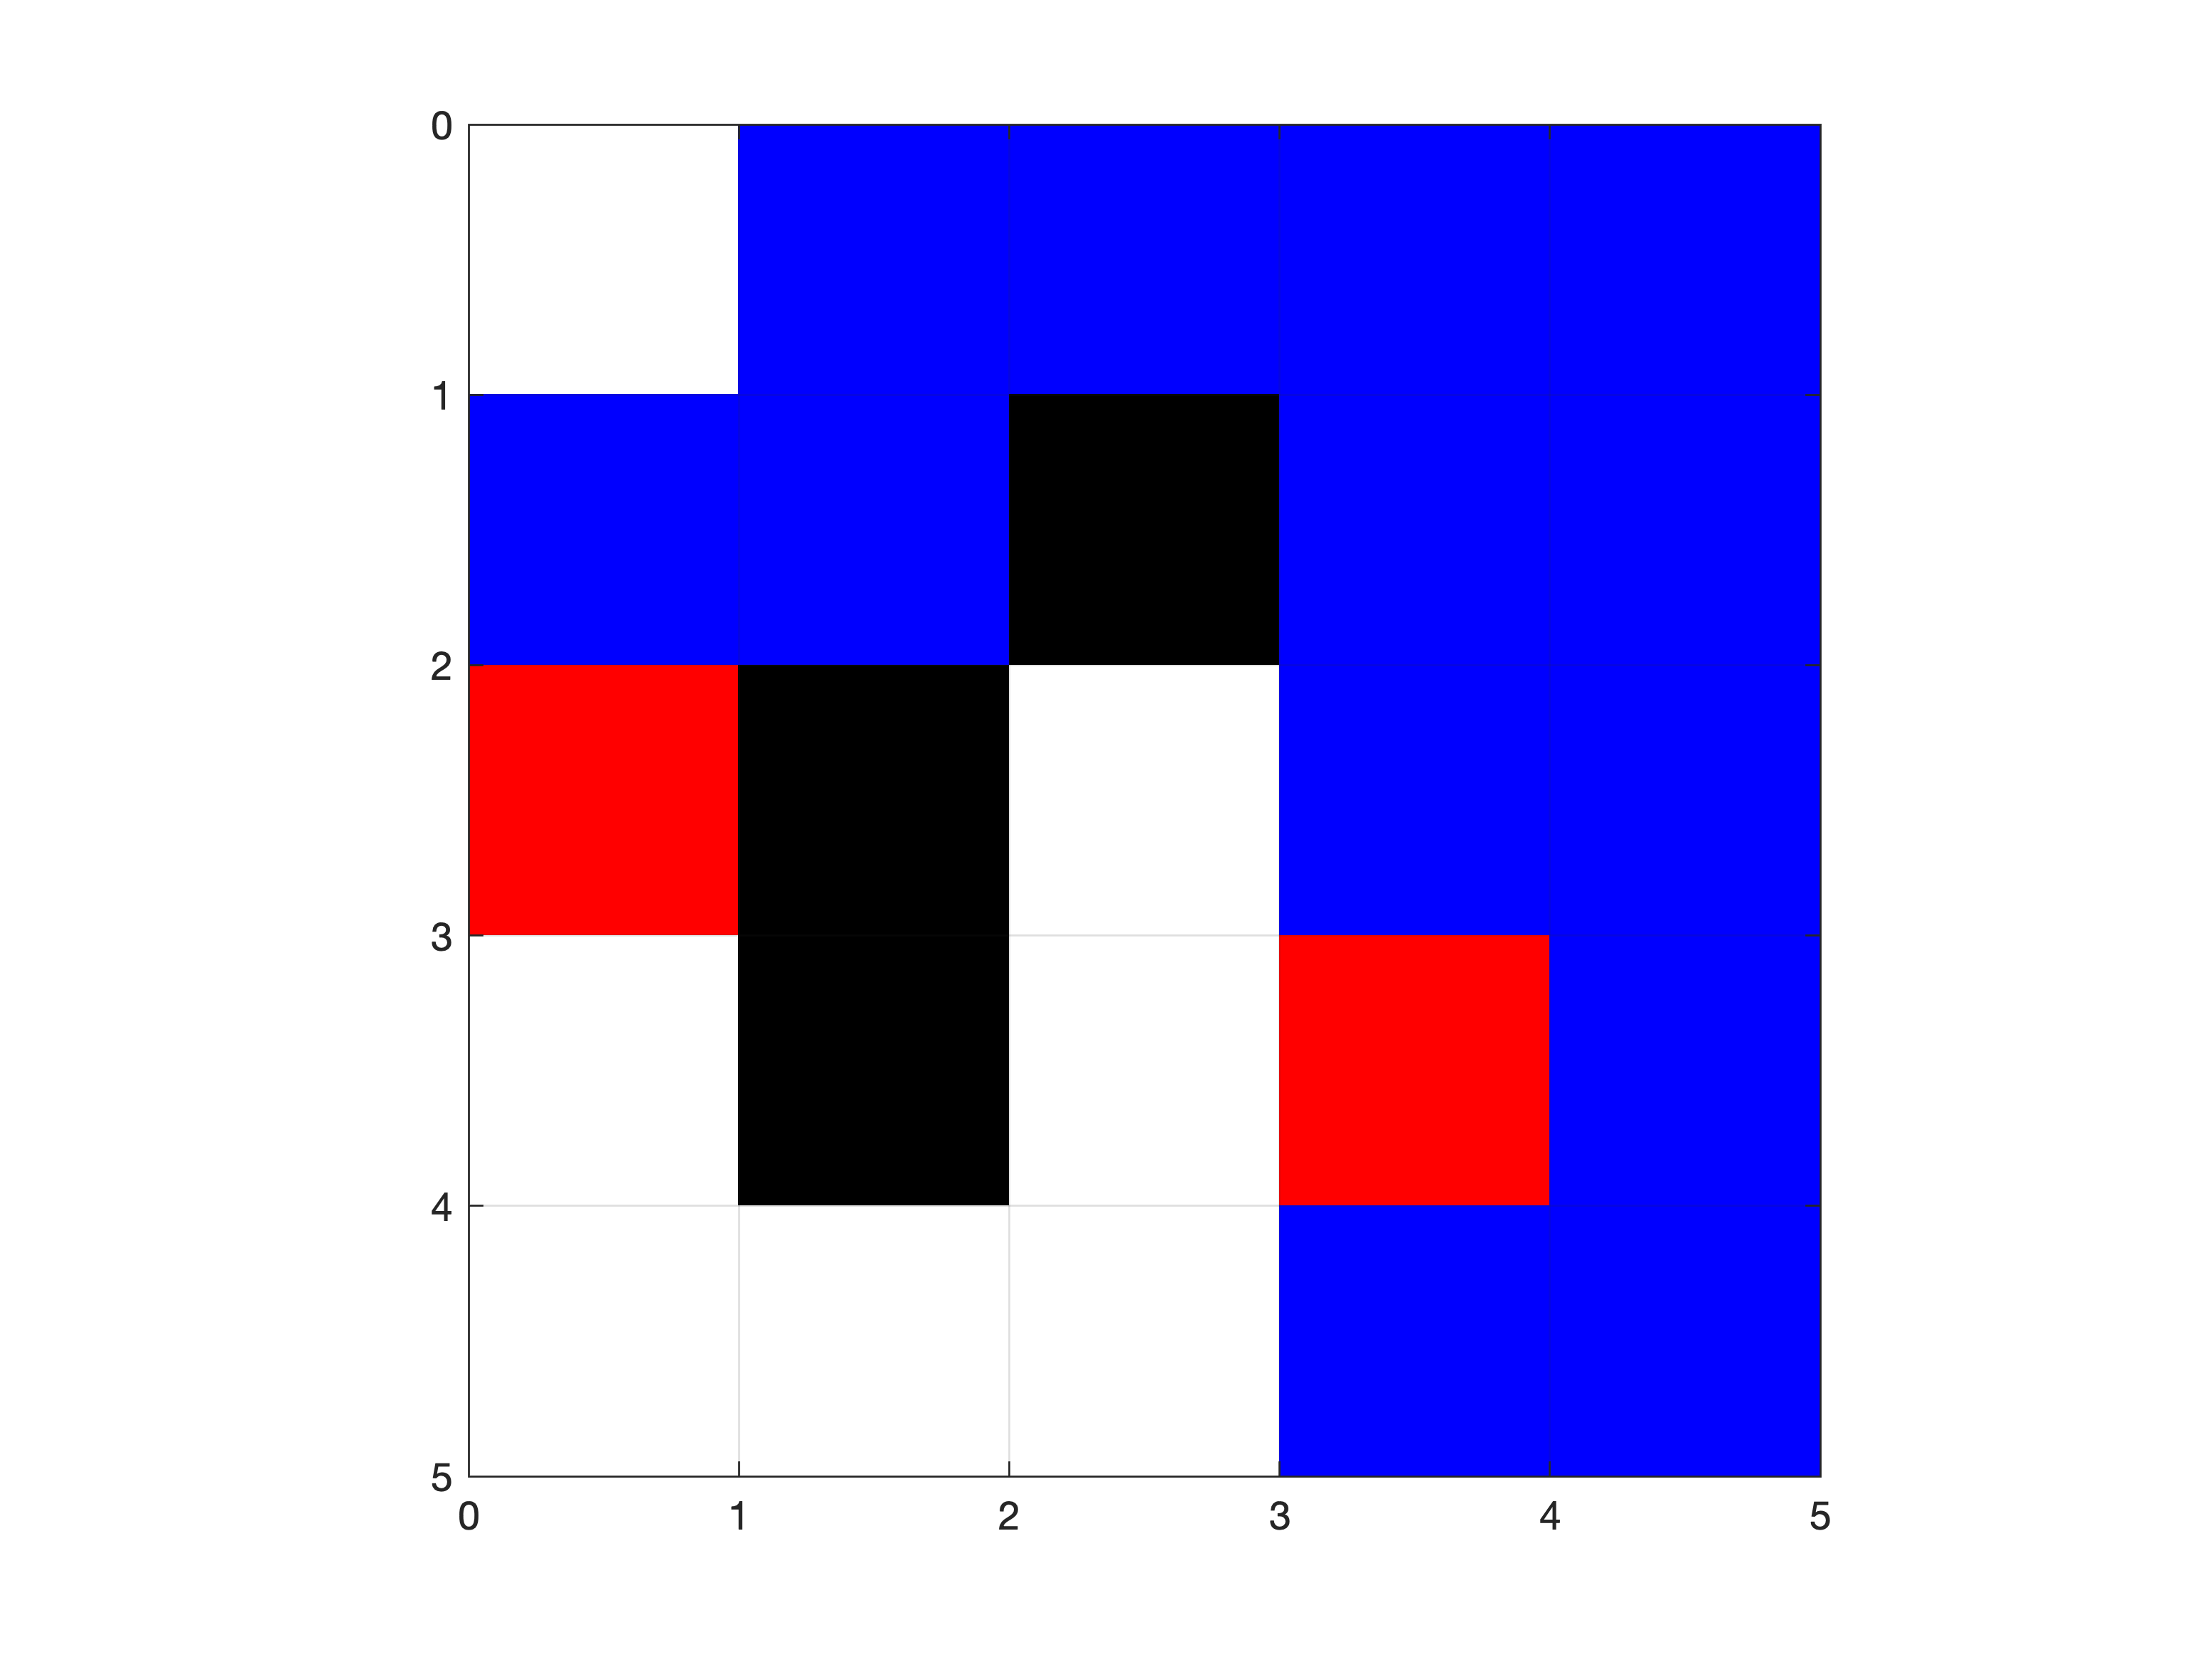
\includegraphics[width=12cm]{../Figure/Q3/50th_path.png}
	\centering
 	\caption{مسیر با هزینه ۱۵ و رتبه ۵۰}
\end{figure}





انیمشین مسیر حرکت نیز در فایل
\lr{map\_visualisation.m}
آورده شده‌است.